\markright{Implementation}
\section{Implementation}
\label{Implementation}
\definecolor{lightgray}{gray}{0.93}
  \vskip\baselineskip%
  \par\noindent\colorbox{lightgray}{%
    \begin{minipage}{0.98\textwidth}
		\textsc{Source Code}:\\
		The extended and working version of the code presented in this paper can be found on:\\
		\texttt{https://github.com/thoeni/rtos-project.git}
		\\There are two branches, the \texttt{main} and the \texttt{icecream} (which has been tested on \texttt{Android 4.0.1\_r1})
    \end{minipage}%
  }%
  \vskip\baselineskip%
As shortly described in the previous section, this small example relies on a native library we'll implement, and a summary of the flow from the Client Application (Activity named BbqueActivity) to the Server (Daemon named bbqued) can be seen in Fig. \ref{fig:projectoverview}.\\
\begin{figure}[!htb]
	\centering
	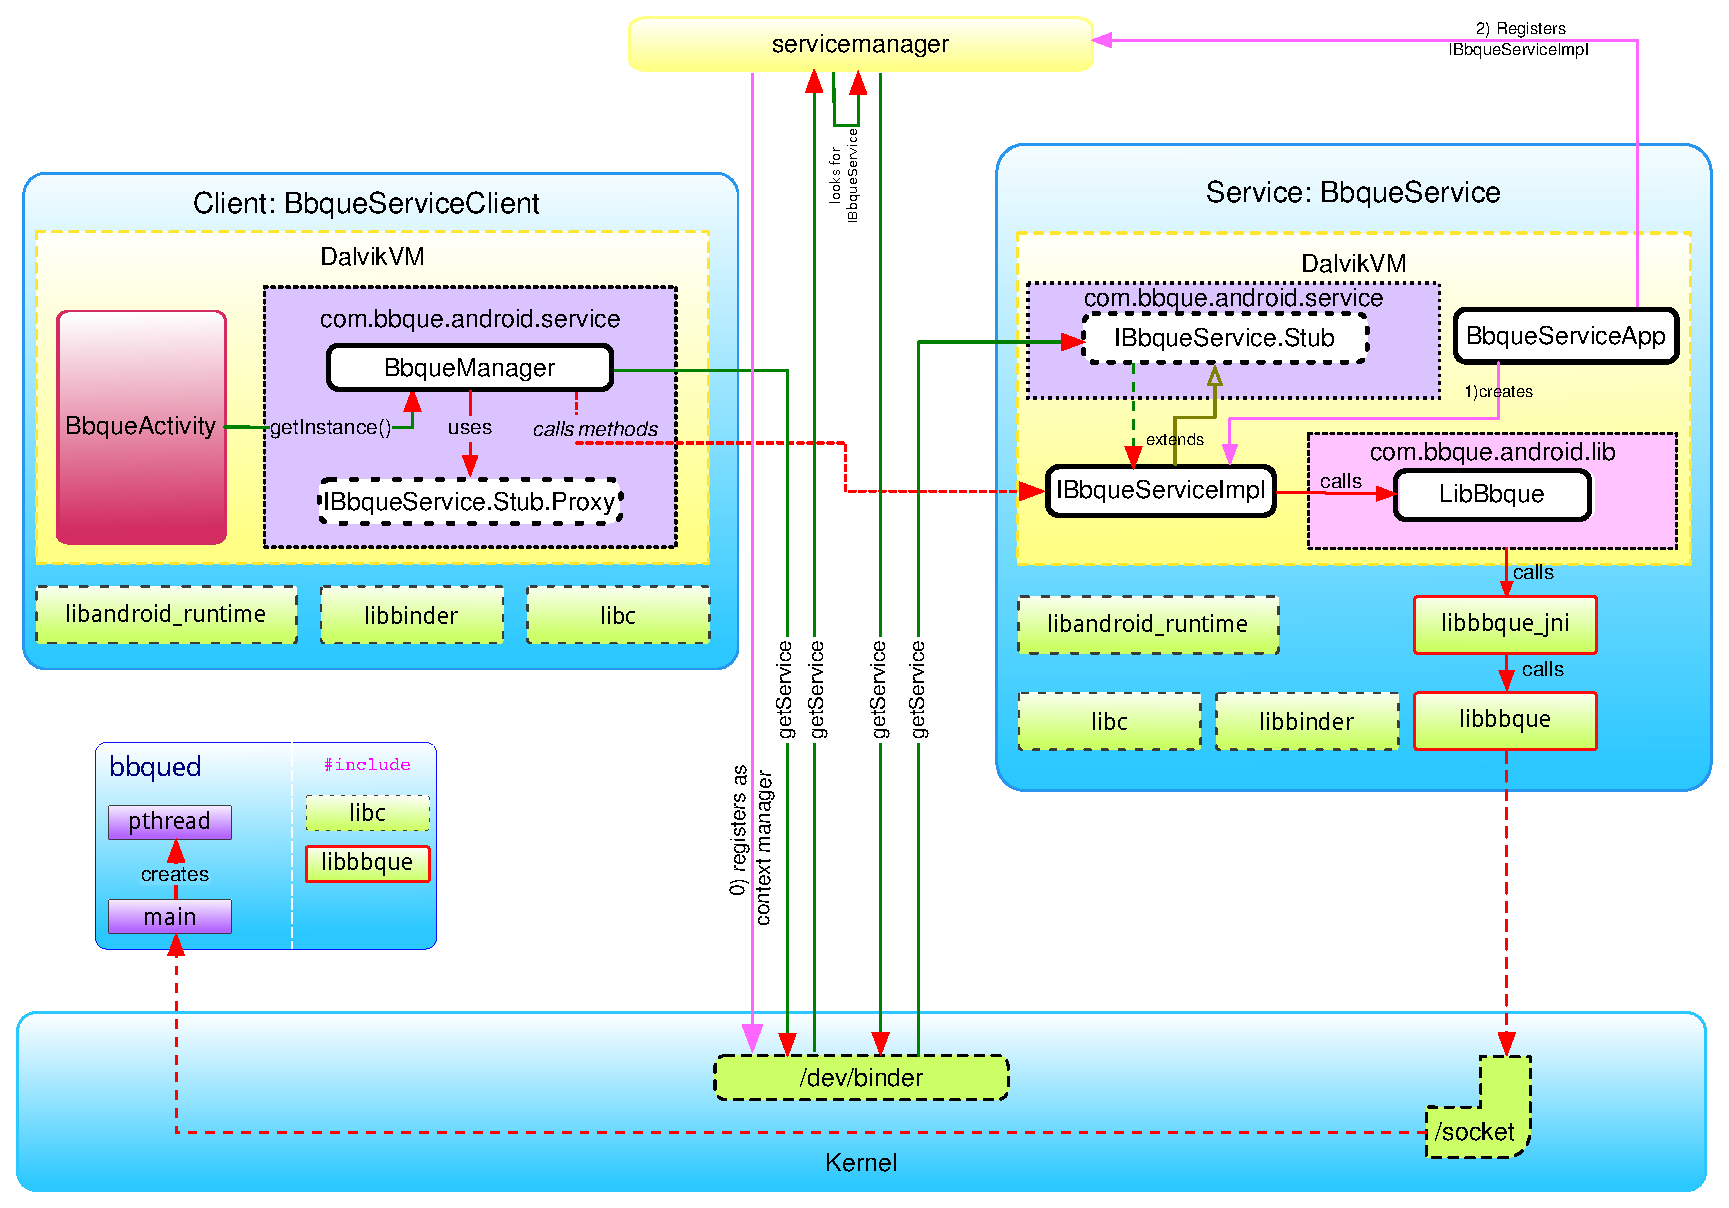
\includegraphics[scale=.432]{images/project_overview.pdf}
	\caption{Project flow overview}
	\label{fig:projectoverview}
\end{figure}
As a very high level consideration, the modules on a \textbf{light blue} background run natively, while the modules over a \textbf{yellow} background run under Dalvik (therefore Java-coded). The \textbf{green} boxes are libraries, and the ones with a red stroke are included by our project. The \textbf{lilac} boxes are the two parts of our service, that communicate each other through binder. The \textbf{pink} box represents the Java module corresponding to our native library: the glue between them comes from JNI code. The flow indicated by the numbered \textbf{pink arrows} is executed during the startup phase.
\subsection{Native library}
Working directory for native library is \texttt{device/bosp/p2012-common/lib}.
The source tree for this directory is
\begin{verbatim}
lib/
├── Android.mk
└── libbbque/
    ├── Android.mk
    ├── libbbque.c
    └── libbbque.h
\end{verbatim}
The outermost \texttt{Android.mk} file contains just the instruction - for the building system - to search deeper for other \textit{makefiles}
\begin{verbatim}
	include $(call all-subdir-makefiles)
\end{verbatim}
The \texttt{libbbque} folder contains the \texttt{.h} header source with library's methods, \texttt{.c} source with library's methods implementation, along with another \texttt{Android.mk} file, which tells to the building system how to build this library module (eg. indicates the source file, the shared libraries to include, the name of the module, its optionality, and so on).\\
For the sake of clarity, we'll consider as example the
\begin{verbatim}
extern int get_core_availability() {
   [...]
   send_message_to_bbqued ("core", &core_number);
   return core_number;
}
\end{verbatim}
the inner method connects to the \texttt{bbqued} daemon through a socket, and sends his message, for instance the string \texttt{"core"}, saving the server's response into \texttt{int core\_number} variable.\\
To register the library module to the system, so that we can - natively - access to it, it's necessary to add to the \texttt{/p2012-common/bosp\_p2012.mk} the following line:
\begin{verbatim}
[...]
PRODUCT_PACKAGES += libbbque
\end{verbatim}
This line will append to the list of other \texttt{PRODUCT\_PACKAGES} string, our customised module, that will be added to the build-to-be version of Android.\\
The library can now be built, potentially as a stand-alone make operation, as follows:
\begin{verbatim}
$ . build/envsetup.sh
$ lunch full_bosp_p2012-eng
$ export USE_CCACHE=1
$ make -j8 libbbque
\end{verbatim}
\subsection{Native daemon}
Working directory for native daemon is \texttt{device/bosp/p2012-common/bin}.
\begin{verbatim}
bin/
├── Android.mk
├── bbqued/
│   ├── Android.mk
│   └── bbqued.c
\end{verbatim}
The outermost \texttt{Android.mk} file is identical to the \texttt{lib/} case, while the inner one contains instructions to properly build the daemon module.\\
The \texttt{bbqued.c} file, which imports the \texttt{libbque.h} library, implements the server side of our test, which creates a \textit{socket} and waits for any incoming connection. When a connection is received, it launches a thread (implemented by using \texttt{pthread} library): each thread reads/writes an \texttt{int} variable which is local to the main process. As done for the library, the daemon module must be added to the \texttt{/p2012-common/bosp\_p2012.mk} file:
\begin{verbatim}
[...]
PRODUCT_PACKAGES += bbqued
\end{verbatim}
\definecolor{lightgray}{gray}{0.93}
  \par\noindent\colorbox{lightgray}{%
    \begin{minipage}{0.98\textwidth}
		\textsc{Adding the process to} \texttt{init.d}:\\
		After building the system, will be possible to run the daemon by accessing the system through \texttt{adb shell} command, and running the \texttt{bbqued} command (since it will be placed straight into \texttt{/bin} folder.\\
		If you want your process to be started at system startup, you can add it to the \texttt{init.d} file that you should have copied before as follows
		\vskip\baselineskip%
		\texttt{\$ cp system/core/rootdir/init.rc device/bosp/p2012-common/.}
		\vskip\baselineskip%	
		Then the building system must be notified to copy this customised file to the target \texttt{root} directory, as follows:
		\vskip\baselineskip%		
		\texttt{PRODUCT\_COPY\_FILES += \$(MY\_PATH)/init.rc:root/init.rc}
    \end{minipage}%
  }%
  \vskip\baselineskip%
To build this module, we have to make the system, as usual.
\subsection{Wrapping native library with JNI}
JNI is the glue to let C and Java talking to each other. This code will be put into directory \texttt{/p2012-common/framework/}, divided int two sub-directories as follows:
\begin{verbatim}
bbque_jni/
|---Android.mk
|---java/
|   |---Android.mk
|   |---com/
|   |   |---bbque/
|   |       |---android/
|   |           |---lib/
|   |               |---LibBbqueException.java
|   |               |---LibBbque.java
|   |---com.bbque.android.lib.xml
|---jni/
    |---Android.mk
    |---com_bbque_android_lib_LibBbque.c
    |---com_bbque_android_lib_LibBbque.h
\end{verbatim}
Create the \texttt{LibBbque.java} class, which contains just the declarations of the methods we want to expose to Java world (which must be declared as \texttt{public native}), as follows:
\begin{verbatim}
public native static int getNumCore() throws LibBbqueException;
\end{verbatim}
and the declaration of the jni library:
\begin{verbatim}
static {
   System.loadLibrary("bbque_jni");
}
\end{verbatim}
The \texttt{xml} file contains the declaration of permissions for the library, that will be generated as \texttt{jar} file during the next step:
\begin{verbatim}
<library name="com.bbque.android.lib"
    file="/system/framework/com.bbque.android.lib.jar"/>
\end{verbatim}
And finally the \texttt{Android.mk} file, under \texttt{java/} directory, h whicis quite elaborate, states all the instructions to properly compile the whole module that will be therefore included into the build process.\\
Then, the \texttt{make} command will process the module, and will generate a \texttt{classes.jar} file, which is needed by the next step, as input parameter to the \texttt{javah -jni} command, that generates the JNI header file.
\begin{verbatim}
$ javah -jni \
        -d device/bosp/p2012-common/framework/bbque_jni/jni/ \
        -classpath out/target/common/obj/JAVA_LIBRARIES/\ 
        com.bbque.android.lib_intermediates/classes-full-debug.jar \
        com.bbque.android.lib.LibBbque
\end{verbatim}
The first line suggests where the output header file will be placed, the second line gives as input the jar shared library generated during the previous step.\\
An example of an auto-generated signature, within the header file, is
\begin{verbatim}
JNIEXPORT jint JNICALL Java_com_bbque_android_lib_LiBbque_getNumCore
  (JNIEnv *, jclass);
\end{verbatim}
The next step consists into the implementation of the header file just generated, for example as follows:
\begin{verbatim}
JNIEXPORT jint JNICALL Java_com_bbque_android_lib_LiBbque_getNumCore
  (JNIEnv *env, jclass clazz) {
  jint result = get_core_availability();
  [...]
  }
\end{verbatim}
It's easy to realize that this is just a wrapping of the C native library.\\
After properly compiling the usual configuration files, \texttt{Android.mk} and the main \textit{makefile} \texttt{bosp\_p2012.mk} with the new modules to include, the system can be built again, and the native library is now accessible through \texttt{LibBbque} class:
\begin{verbatim}
LibBbque.getNumCore();
\end{verbatim}
We can say that the java call, so far, works within the upper right part of Fig. \ref{fig:projectoverview}, by calling Java methods on the \texttt{LibBbque} class (pink box).